
\section{DSP-spezifische Optimierung der implementierten Merkmalsextraktion}\label{sec:optdsp}
F�r die Merkmalsextraktion auf dem C674x DSP wurde eine C-Version der C++-Referenz-Klasse geschrieben. da der Compiler C++ nur in geringem Umfang unterst�tzt. Au�erdem wurde f�r die Einbindung der Merkmalsextraktion in den ARM-Code C6Runlib gew�hlt, da f�r C6Runapp keine Komunikationsprotokolle definiert sind.\\
Die Laufzeiten zur Extraaktion der Merkmale und zur Durchf�hrung erforderlicher Algorithmen sin in \textbf{Abbildung \ref{fig:startdsp}}zu sehen.\\
%
\begin{figure}[h]
	\centering
		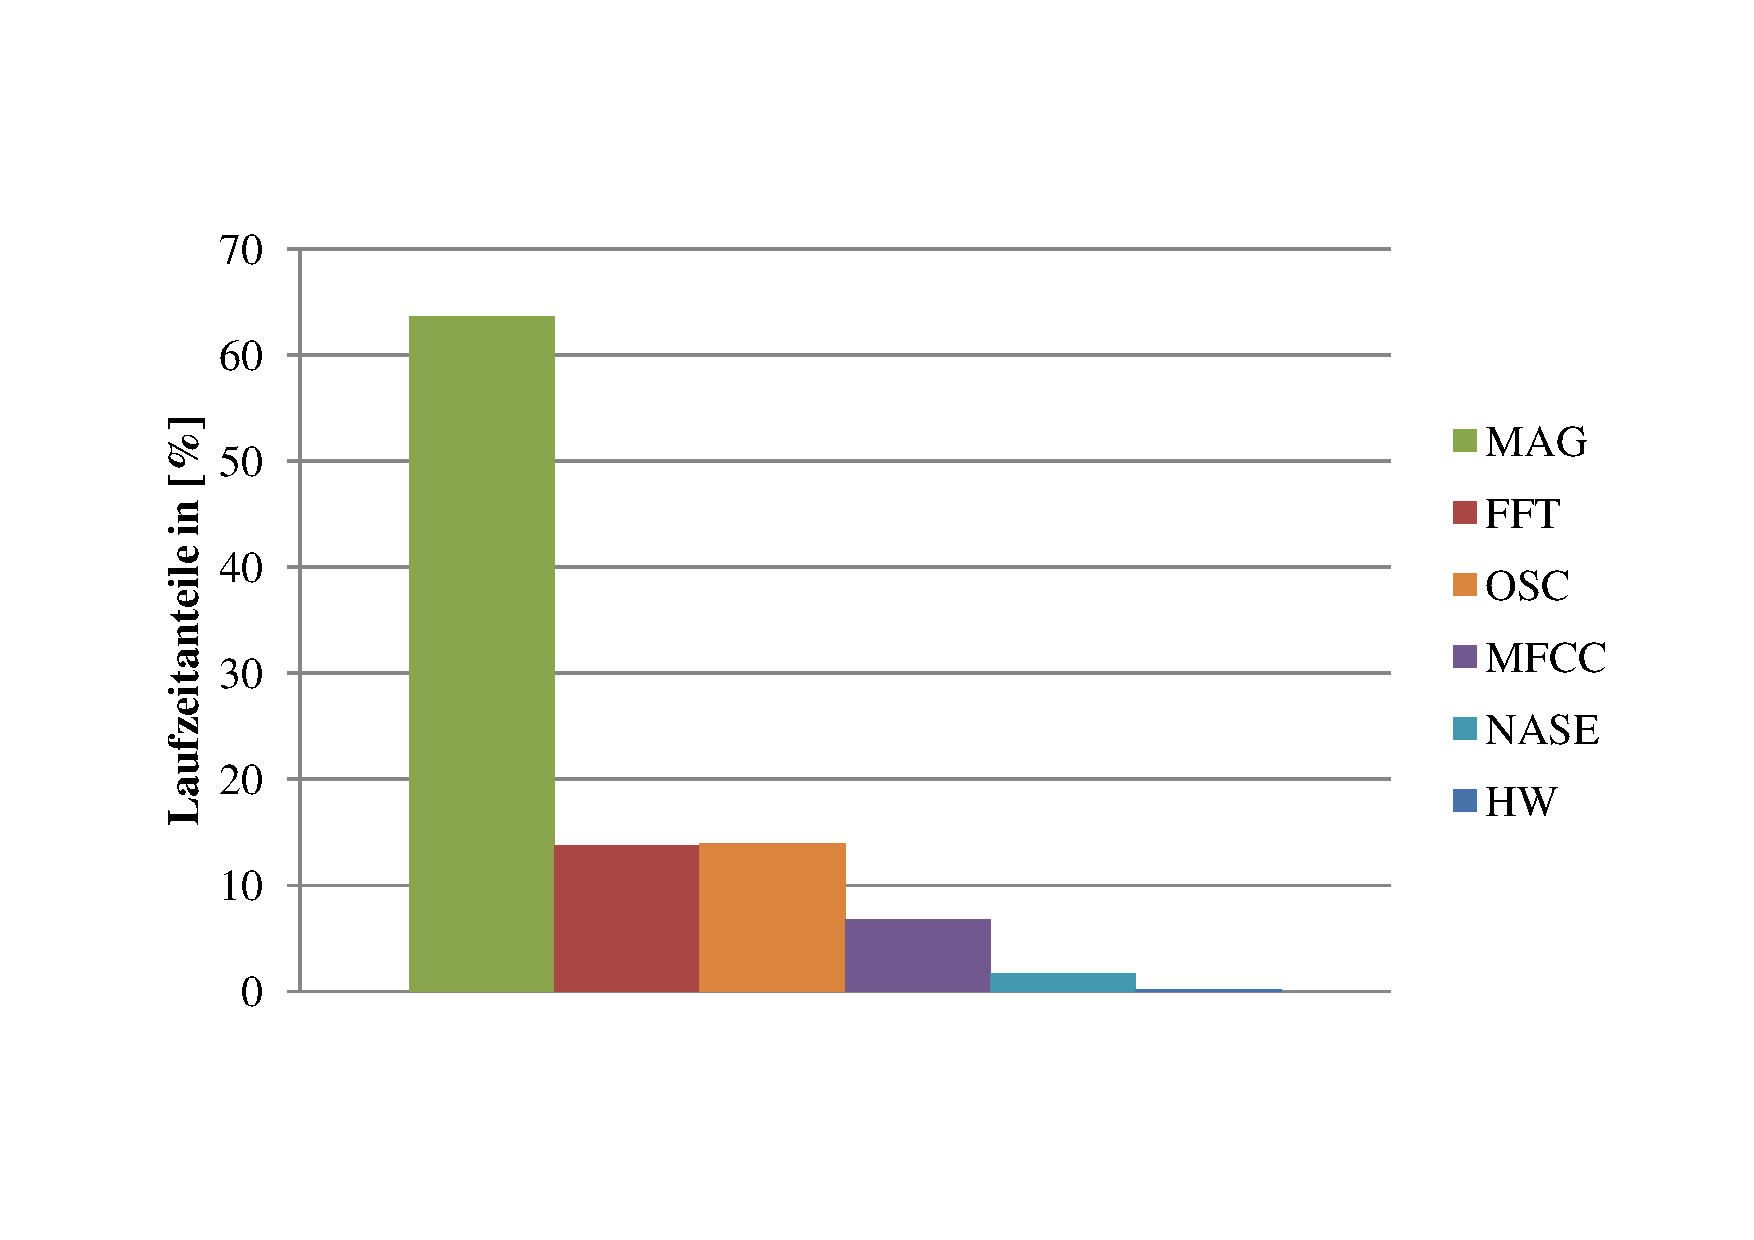
\includegraphics[width=1\textwidth]{../Pictures/startdsp.pdf}
	\caption{Laufzeitanteile der einzelnen Features}
	\label{fig:startdsp}
\end{figure} 
%
Wie der Abbildung entnommen werden kann, f�llt der gr��te Anteil der Ausf�hrungszeit mit �ber 60\% der MAG-Berechnung zu.\\

\subsection{Optimierung der Rechenfunktionen mit MATHLIB}\label{sec:mathlib}
Eine genaue Analyse der Laufzeit der MAG-Berechnung zeigt, dass 98\% der Verarbeitungszeit auf die Berechnung der Division und Wurzelberechnung fallen, die mehrfach ausgef�hrt werden. Zur Beschleunigung dieser Operationen eignen sich die MATHLIB-Funktionen f�r vektorielle Eingabewerte.\\
\textbf{Listing \ref{code:aoscc}} zeigt den Referenz-Code der MAG-Berechnung und \textbf{Listing \ref{code:aoscm}} durch MATHLIB optimierten Code.

\begin{lstlisting}[caption=Referenzcode von Magnitude of Spectrum, label=code:aoscc]
	A[k] = sqrt(X[k] * X[k] + Y[k] * Y[k]) / G;
\end{lstlisting}

\begin{lstlisting}[caption=Magnitude of Spectrum mit MATHLIB, label=code:aoscm]
	for (k = 0; k < G; ++k) {
		tmp1 = X[k] * X[k];
		tmp2 = Y[k] * Y[k];
		A[k] = (tmp1 + tmp2); //(X[k] * X[k] + Y[k] * Y[k]);
	}
	
	sqrtsp_v(A, A, G);

	divsp_v(A, pG, A, G);
\end{lstlisting}

Hierbei ist zu erw�hnen, dass die Addition innerhalb der Wurzelberechnung wird zus�tzlich f�r eine bessere Ausf�hrung durch SPLOOP aufgetrennt wird.\\
Mit dieser Optimierung wird f�r FSet 1 und 4 eine Beschleunigung um den Faktor 45,5 und bei FSet2 um 45,2 erreicht.\\
Die MATHLIB wird au�erdem f�r die Optimierung folgender Algorithmen eingesetzt:

\begin{itemize}
\item MFCC
\item Low Energy
\item Normalized Audio Spectrum Envelope
\item Octave Spectral Contrast
\item Root Mean Square
\item Spectral Centroid
\item Spectral Crest Factor
\item Spectral Flux
\item Sub-band Energy Ratio
\end{itemize}

Die Beschleunigungen dieser Merkmale ist in \textbf{Tabelle \ref{tab:math}} angegeben.

\begin{table*}[ht]
	\centering
		\begin{tabular}{c|c|c|c|c|c|c|c|c|c}
		
		& MFCC & LE & NASE & OSC & RMS & SC & SCF & SF & SBER\\
		\hline
		Faktor & 3 & 2,4 & 2,2 & 2,2 & 1,3 & 1,4 & 2,2 & 1,05 & 1,8\\
					
		\end{tabular}
	\caption{Tabelle der verwendeten Ausdr�cke und Variablen}
	\label{tab:math}
\end{table*}

Insgesamt werden durch die Einbindung von MATHLIB die FSets 1, 2, 3 und 4 um die Faktoren 4.6, 4.1, 1.1 und 4.7 beschleunigt.

\begin{figure}[h]
	\centering
		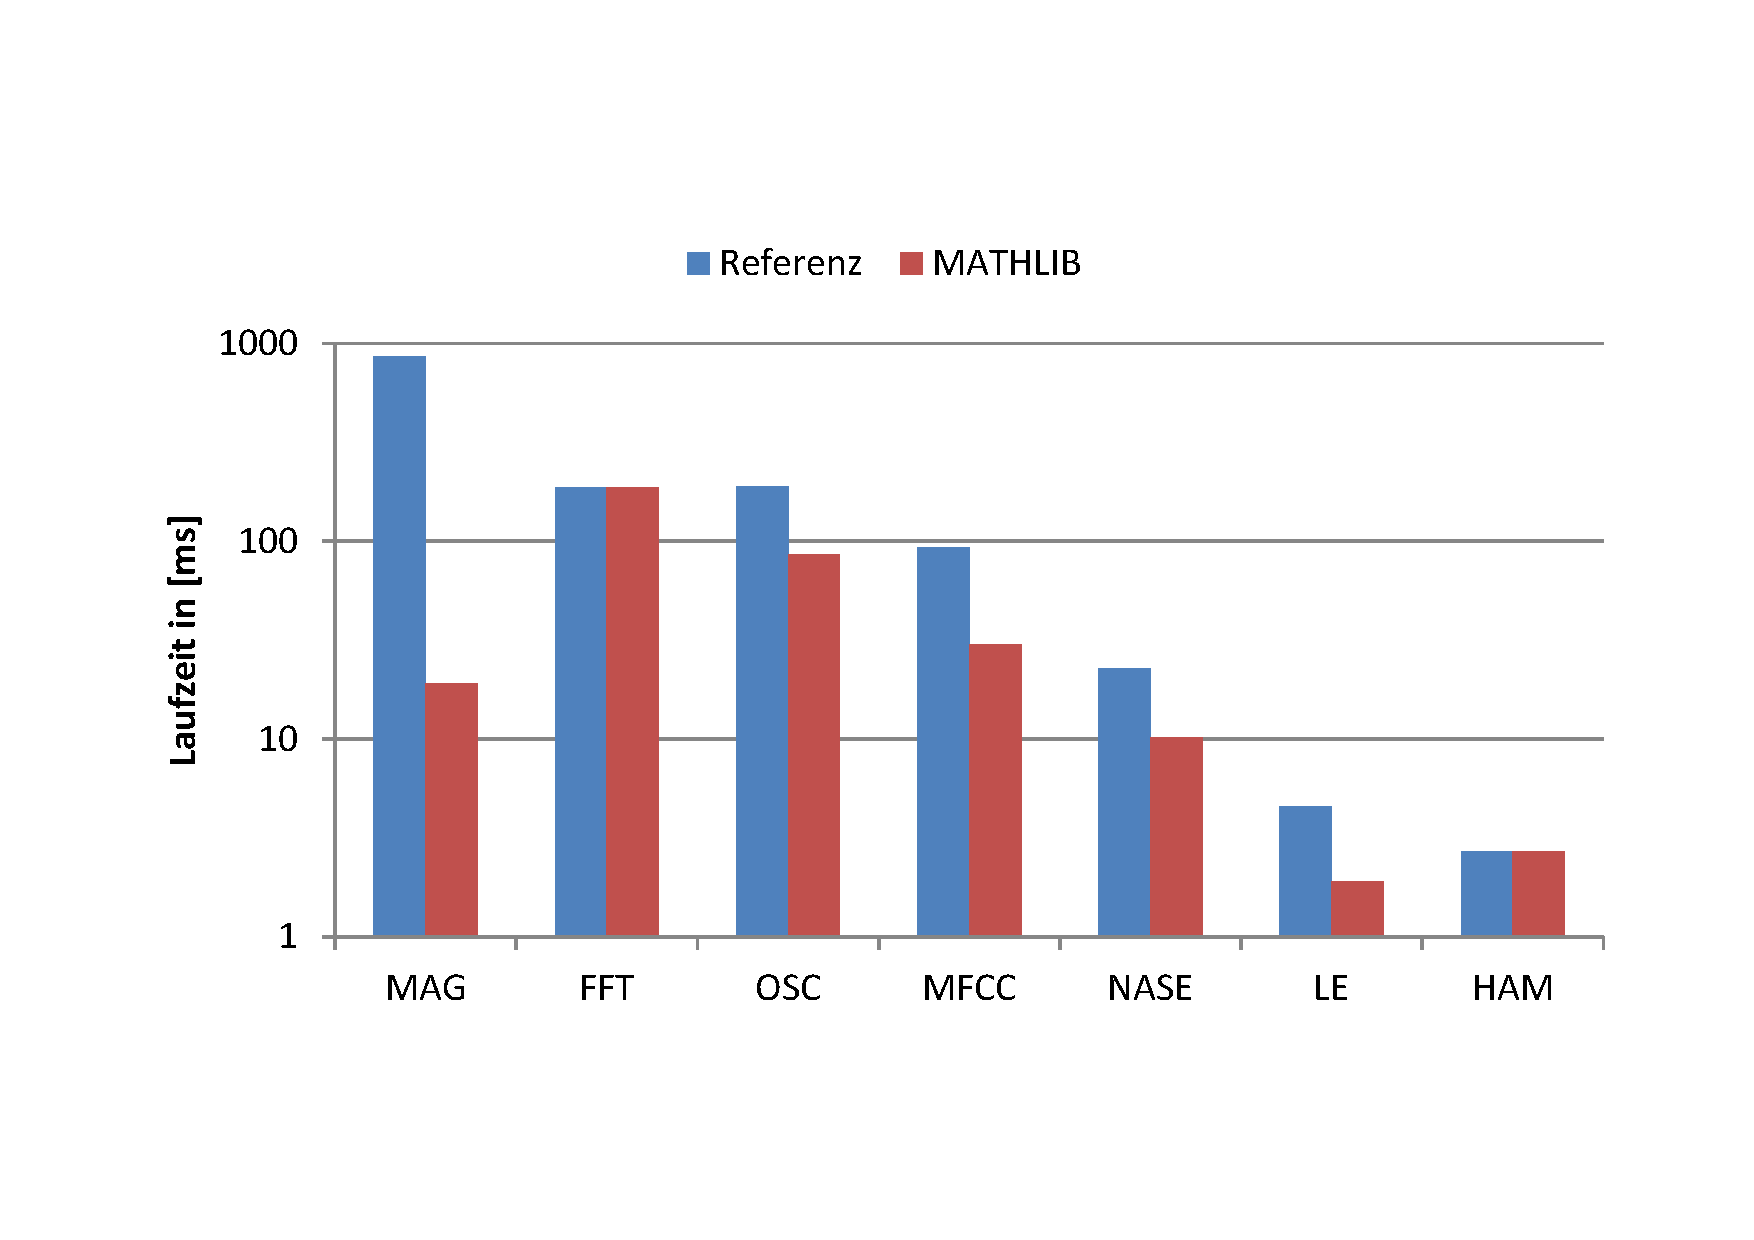
\includegraphics[width=1\textwidth]{../Pictures/dsp2.pdf}
	\caption{Laufzeitmessung nach der Optimierung durch MATHLIB}
	\label{fig:dsp2}
\end{figure} 
%
\textbf{Abbildung \ref{fig:dsp2}} veranschaulicht die Laufzeit-Verbesserungen der Merkmale durch die MATHLIB.\\
Des weiteren f�llt auf, dass die FFT-Berechnung nun die l�ngste Laufzeit aufweist.

\subsection{Optimierung der FFT mit DSPLIB}\label{sec:dsplib}
Die Beschleunigung der FFT wird mit Hilfe der DSPLIB-Implementierung realisiert. Hierbei wird der Programm-Code der MAG aufgrund des ge�nderten Datenformats angepasst.\\
Dieses beschleunigt die FFT-Berechnung f�r FSet 1, 2 und 4 je um den Faktor 3,8. Insgesamt werden die FSets 1, 2 und 4 zus�tzlich um die Faktoren 2, 1,6 und 2,2 beschleunigt.\\
Nach der Optimierung mit der DSPLIB sind die Berechnungen der Merkmale OSC und ZCR langsamer als die Berechnung der FFT.

\subsection{Optimierung des Sortierverfahrens der Octave Spectral Contrast-Berechnung}\label{subsec:optosc}
Eine genauere Analyse der Berechnung des OSC-Merkmals zeigt, dass 54\% der Rechenzeit dieses Merkmals auf die Sortierung fallen. Also wird eine Optimierung des Sortierverfahrens angestrebt.\\
Bei dem im Referenz-Code verwendeten Sortierverfahren handelt es sich um einen Algorithmus, der auf dem Quick Sort-Verfahren basiert. Nach Angaben von Texas Instruments\cite{sort} werden Merge Sort-Algorithmen auf dem C674x DSP laufezeiteffektiver ausgef�hrt, als Quick Sort-Algorithmen, obwohl beide in die  Komplexit�tsklasse $O(n \, log(n))$ fallen. In dem selben Dokument wird ebenfalls ein optimierter Algorithmus auf dem Merge Sort-Verfahren basierend pr�sentiert. Dieser f�r Integer konzipierte Algorithmus wird f�r die Verwendung mit Flie�punktzahlen und die Sortierung in absteigender Reihenfolge umgeschrieben und in die OSC-Berechnung integriert.\\
Die Ersetzung des Quick Sort-Verfahrens durch das in \cite{sort} vorgeschlagene Merge Sort-Verfahren beschleunigt die Berechnung des OSC-Merkmals um den Faktor 1,1 . Insgesamt wird hierdurch die Berechnung von FSet2 um den Faktor 1,05 beschleunigt.

\subsection{Optimierung f�r SPLOOP}\label{sec:compiler} 
Ein Blick in den Assemblercode der Zero Crossing Rate zeigt, dass f�r die Schleife keine SPLOOP-Optimierung vom Compiler durchgef�hrt wurde. Dieses l�sst sich aber durch eine einfache Codeumstellung l�sen. \textbf{Listing \ref{code:zcrc}} zeigt den Referenzcode der Zero Crossing Rate und \textbf{Listing \ref{code:zcrs}} den umgestellen Code.

\begin{lstlisting}[caption=Referenzcode der Schleife der Zero Crossing Rate, label=code:zcrc]
	for (n = 0; n < zinfo.N - 1; ++n) {
		zero_crossings += ABS(SGN(signal[n])-SGN(signal[n+1]));
	}
\end{lstlisting}

\begin{lstlisting}[caption=F�r SPLOOP umgestellter Code der Schleife der Zero Crossing Rate, label=code:zcrs]
	for (n = 0; n < zinfo.N - 1; ++n) {
		tsgn1 = SGN(signal[n]);

		tsgn2 = SGN(signal[n+1]);

		tsub = tsgn1 - tsgn2;

		tabs = ABS(tsub);

		zero_crossings += tabs;
	}
\end{lstlisting}

Die Code-Umstellung beschleunigt die ZCR-Berechnung um einen Faktor von 7,7, so dass die Berechnung von FSet3 um den Faktor 3,9 beschleunigt wird.